
\begin{figure}[H]
\centering
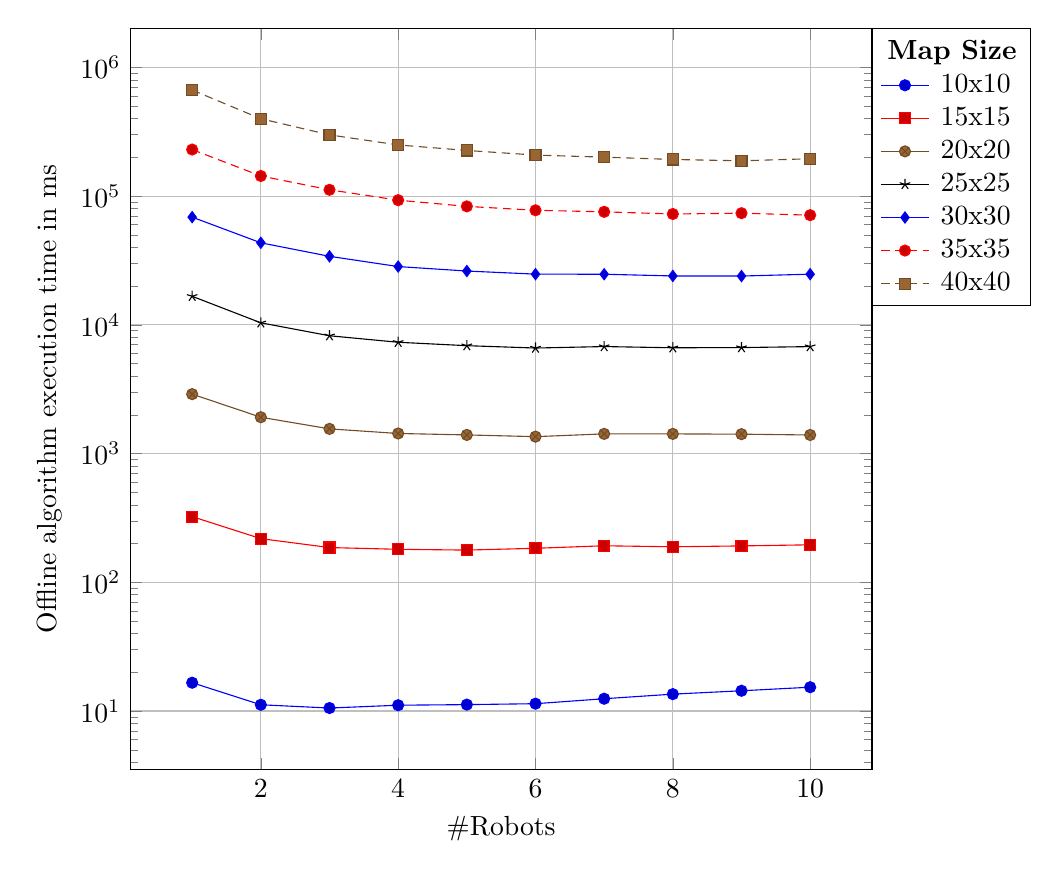
\begin{tikzpicture}
	\begin{semilogyaxis}[
		height=11cm,
		width=11cm,
                legend style = {at={(1,1)}, anchor=north west},
		grid=major,
		xlabel=\#Robots,
                   ylabel=Offline algorithm execution time in ms
	]

        \addlegendimage{empty legend}
        \addlegendentry{\hspace{-.6cm}\textbf{Map Size}}

%	\addplot coordinates {
%		(1, 0.962165)
%		(2, 0.999812)
%		(3, 3.32455)
%		(4, 1.33711)
%		(5, 1.26769)
%		(6, 4.00359)
%		(7, 4.45941)
%		(8, 1.33102)
%		(9, 1.38427)
%                (10, 3.06631)
%	};
%	\addlegendentry{5x5}

	\addplot coordinates {
		(1, 99.5812/6)
		(2, 67.1215/6)
		(3, 63.3223/6)
		(4, 66.5972/6)
		(5, 67.303/6)
		(6, 68.4257/6)
		(7, 74.7808/6)
		(8, 81.1845/6)
		(9, 86.226/6)
                (10, 91.9106/6)
	};
	\addlegendentry{10x10}

	\addplot coordinates {
		(1, 1941.57/6)
		(2, 1310.12/6)
		(3, 1117.07/6)
		(4, 1082.52/6)
		(5, 1067.53/6)
		(6, 1102.4/6)
		(7, 1153.16/6)
		(8, 1132.38/6)
		(9, 1150.22/6)
                (10, 1173.2/6)
	};
	\addlegendentry{15x15}

	\addplot coordinates {
		(1, 17361.1/6)
		(2, 11490/6)
		(3, 9328.54/6)
		(4, 8591.75/6)
		(5, 8372.56/6)
		(6, 8116.5/6)
		(7, 8529.95/6)
		(8, 8526.77/6)
		(9, 8485.28/6)
                (10, 8361.64/6)
	};
	\addlegendentry{20x20}

	\addplot coordinates {
		(1, 99929.9/6)
		(2, 62180.2/6)
		(3, 49326.2/6)
		(4, 43910.5/6)
		(5, 41311.1/6)
		(6, 39607.3/6)
		(7, 40667/6)
		(8, 39792/6)
		(9, 39942.7/6)
                (10,40629.5/6)
	};
	\addlegendentry{25x25}

	\addplot coordinates {
		(1, 411589/6)
		(2, 260044/6)
		(3, 204265/6)
		(4, 170023/6)
		(5, 156969/6)
		(6, 148516/6)
		(7, 148225/6)
		(8, 143764/6)
		(9, 143510/6)
                (10, 148387/6)
	};
	\addlegendentry{30x30}

	\addplot coordinates {
		(1, 1.37889e+06/6)
		(2, 859312/6)
		(3, 671124/6)
		(4, 557420/6)
		(5, 498969/6)
		(6, 465257/6)
		(7, 452598/6)
		(8, 435339/6)
		(9, 441815/6)
                (10, 426400/6)
	};
	\addlegendentry{35x35}

	\addplot coordinates {
		(1, 3.99748e+06/6)
		(2, 2.39203e+06/6)
		(3, 1.79249e+06/6)
		(4, 1.49702e+06/6)
		(5, 1.35637e+06/6)
		(6, 1.24861e+06/6)
		(7, 1.20327e+06/6)
		(8, 1.15456e+06/6)
		(9, 1.12716e+06/6)
                (10, 1.16961e+06/6)
	};
	\addlegendentry{40x40}
	
	\end{semilogyaxis}
\end{tikzpicture}
\caption{VRP-FloydWarshall:  Different execution times for growing map sizes}
\label{fig:VRPFW_execTime}
\end{figure}

